
%% bare_jrnl.tex
%% V1.3
%% 2007/01/11
%% by Michael Shell
%% see http://www.michaelshell.org/
%% for current contact information.
%%
%% This is a skeleton file demonstrating the use of IEEEtran.cls
%% (requires IEEEtran.cls version 1.7 or later) with an IEEE journal paper.
%%
%% Support sites:
%% http://www.michaelshell.org/tex/ieeetran/
%% http://www.ctan.org/tex-archive/macros/latex/contrib/IEEEtran/
%% and
%% http://www.ieee.org/



% *** Authors should verify (and, if needed, correct) their LaTeX system  ***
% *** with the testflow diagnostic prior to trusting their LaTeX platform ***
% *** with production work. IEEE's font choices can trigger bugs that do  ***
% *** not appear when using other class files.                            ***
% The testflow support page is at:
% http://www.michaelshell.org/tex/testflow/


%%*************************************************************************
%% Legal Notice:
%% This code is offered as-is without any warranty either expressed or
%% implied; without even the implied warranty of MERCHANTABILITY or
%% FITNESS FOR A PARTICULAR PURPOSE! 
%% User assumes all risk.
%% In no event shall IEEE or any contributor to this code be liable for
%% any damages or losses, including, but not limited to, incidental,
%% consequential, or any other damages, resulting from the use or misuse
%% of any information contained here.
%%
%% All comments are the opinions of their respective authors and are not
%% necessarily endorsed by the IEEE.
%%
%% This work is distributed under the LaTeX Project Public License (LPPL)
%% ( http://www.latex-project.org/ ) version 1.3, and may be freely used,
%% distributed and modified. A copy of the LPPL, version 1.3, is included
%% in the base LaTeX documentation of all distributions of LaTeX released
%% 2003/12/01 or later.
%% Retain all contribution notices and credits.
%% ** Modified files should be clearly indicated as such, including  **
%% ** renaming them and changing author support contact information. **
%%
%% File list of work: IEEEtran.cls, IEEEtran_HOWTO.pdf, bare_adv.tex,
%%                    bare_conf.tex, bare_jrnl.tex, bare_jrnl_compsoc.tex
%%*************************************************************************

% Note that the a4paper option is mainly intended so that authors in
% countries using A4 can easily print to A4 and see how their papers will
% look in print - the typesetting of the document will not typically be
% affected with changes in paper size (but the bottom and side margins will).
% Use the testflow package mentioned above to verify correct handling of
% both paper sizes by the user's LaTeX system.
%
% Also note that the "draftcls" or "draftclsnofoot", not "draft", option
% should be used if it is desired that the figures are to be displayed in
% draft mode.
%
\documentclass[journal]{IEEEtran}
\usepackage{blindtext}
\usepackage{graphicx}
\graphicspath{ {images/} }
\usepackage{array}
\newcolumntype{L}[1]{>{\raggedright\let\newline\\\arraybackslash\hspace{0pt}}m{#1}}

% *** CITATION PACKAGES ***
%
%\usepackage{cite}
% cite.sty was written by Donald Arseneau
% V1.6 and later of IEEEtran pre-defines the format of the cite.sty package
% \cite{} output to follow that of IEEE. Loading the cite package will
% result in citation numbers being automatically sorted and properly
% "compressed/ranged". e.g., [1], [9], [2], [7], [5], [6] without using
% cite.sty will become [1], [2], [5]--[7], [9] using cite.sty. cite.sty's
% \cite will automatically add leading space, if needed. Use cite.sty's
% noadjust option (cite.sty V3.8 and later) if you want to turn this off.
% cite.sty is already installed on most LaTeX systems. Be sure and use
% version 4.0 (2003-05-27) and later if using hyperref.sty. cite.sty does
% not currently provide for hyperlinked citations.
% The latest version can be obtained at:
% http://www.ctan.org/tex-archive/macros/latex/contrib/cite/
% The documentation is contained in the cite.sty file itself.



% *** GRAPHICS RELATED PACKAGES ***
%
\ifCLASSINFOpdf
  % \usepackage[pdftex]{graphicx}
  % declare the path(s) where your graphic files are
  % \graphicspath{{../pdf/}{../jpeg/}}
  % and their extensions so you won't have to specify these with
  % every instance of \includegraphics
  % \DeclareGraphicsExtensions{.pdf,.jpeg,.png}
\else
  % or other class option (dvipsone, dvipdf, if not using dvips). graphicx
  % will default to the driver specified in the system graphics.cfg if no
  % driver is specified.
  % \usepackage[dvips]{graphicx}
  % declare the path(s) where your graphic files are
  % \graphicspath{{../eps/}}
  % and their extensions so you won't have to specify these with
  % every instance of \includegraphics
  % \DeclareGraphicsExtensions{.eps}
\fi
% graphicx was written by David Carlisle and Sebastian Rahtz. It is
% required if you want graphics, photos, etc. graphicx.sty is already
% installed on most LaTeX systems. The latest version and documentation can
% be obtained at: 
% http://www.ctan.org/tex-archive/macros/latex/required/graphics/
% Another good source of documentation is "Using Imported Graphics in
% LaTeX2e" by Keith Reckdahl which can be found as epslatex.ps or
% epslatex.pdf at: http://www.ctan.org/tex-archive/info/
%
% latex, and pdflatex in dvi mode, support graphics in encapsulated
% postscript (.eps) format. pdflatex in pdf mode supports graphics
% in .pdf, .jpeg, .png and .mps (metapost) formats. Users should ensure
% that all non-photo figures use a vector format (.eps, .pdf, .mps) and
% not a bitmapped formats (.jpeg, .png). IEEE frowns on bitmapped formats
% which can result in "jaggedy"/blurry rendering of lines and letters as
% well as large increases in file sizes.
%
% You can find documentation about the pdfTeX application at:
% http://www.tug.org/applications/pdftex



% *** SUBFIGURE PACKAGES ***
%\usepackage[tight,footnotesize]{subfigure}
% subfigure.sty was written by Steven Douglas Cochran. This package makes it
% easy to put subfigures in your figures. e.g., "Figure 1a and 1b". For IEEE
% work, it is a good idea to load it with the tight package option to reduce
% the amount of white space around the subfigures. subfigure.sty is already
% installed on most LaTeX systems. The latest version and documentation can
% be obtained at:
% http://www.ctan.org/tex-archive/obsolete/macros/latex/contrib/subfigure/
% subfigure.sty has been superceeded by subfig.sty.

%\usepackage[caption=false]{caption}
%\usepackage[font=footnotesize]{subfig}
% subfig.sty, also written by Steven Douglas Cochran, is the modern
% replacement for subfigure.sty. However, subfig.sty requires and
% automatically loads Axel Sommerfeldt's caption.sty which will override
% IEEEtran.cls handling of captions and this will result in nonIEEE style
% figure/table captions. To prevent this problem, be sure and preload
% caption.sty with its "caption=false" package option. This is will preserve
% IEEEtran.cls handing of captions. Version 1.3 (2005/06/28) and later 
% (recommended due to many improvements over 1.2) of subfig.sty supports
% the caption=false option directly:
%\usepackage[caption=false,font=footnotesize]{subfig}
%
% The latest version and documentation can be obtained at:
% http://www.ctan.org/tex-archive/macros/latex/contrib/subfig/
% The latest version and documentation of caption.sty can be obtained at:
% http://www.ctan.org/tex-archive/macros/latex/contrib/caption/


% *** FLOAT PACKAGES ***
%
%\usepackage{fixltx2e}
% fixltx2e, the successor to the earlier fix2col.sty, was written by
% Frank Mittelbach and David Carlisle. This package corrects a few problems
% in the LaTeX2e kernel, the most notable of which is that in current
% LaTeX2e releases, the ordering of single and double column floats is not
% guaranteed to be preserved. Thus, an unpatched LaTeX2e can allow a
% single column figure to be placed prior to an earlier double column
% figure. The latest version and documentation can be found at:
% http://www.ctan.org/tex-archive/macros/latex/base/



%\usepackage{stfloats}
% stfloats.sty was written by Sigitas Tolusis. This package gives LaTeX2e
% the ability to do double column floats at the bottom of the page as well
% as the top. (e.g., "\begin{figure*}[!b]" is not normally possible in
% LaTeX2e). It also provides a command:
%\fnbelowfloat
% to enable the placement of footnotes below bottom floats (the standard
% LaTeX2e kernel puts them above bottom floats). This is an invasive package
% which rewrites many portions of the LaTeX2e float routines. It may not work
% with other packages that modify the LaTeX2e float routines. The latest
% version and documentation can be obtained at:
% http://www.ctan.org/tex-archive/macros/latex/contrib/sttools/
% Documentation is contained in the stfloats.sty comments as well as in the
% presfull.pdf file. Do not use the stfloats baselinefloat ability as IEEE
% does not allow \baselineskip to stretch. Authors submitting work to the
% IEEE should note that IEEE rarely uses double column equations and
% that authors should try to avoid such use. Do not be tempted to use the
% cuted.sty or midfloat.sty packages (also by Sigitas Tolusis) as IEEE does
% not format its papers in such ways.


%\ifCLASSOPTIONcaptionsoff
%  \usepackage[nomarkers]{endfloat}
% \let\MYoriglatexcaption\caption
% \renewcommand{\caption}[2][\relax]{\MYoriglatexcaption[#2]{#2}}
%\fi
% endfloat.sty was written by James Darrell McCauley and Jeff Goldberg.
% This package may be useful when used in conjunction with IEEEtran.cls'
% captionsoff option. Some IEEE journals/societies require that submissions
% have lists of figures/tables at the end of the paper and that
% figures/tables without any captions are placed on a page by themselves at
% the end of the document. If needed, the draftcls IEEEtran class option or
% \CLASSINPUTbaselinestretch interface can be used to increase the line
% spacing as well. Be sure and use the nomarkers option of endfloat to
% prevent endfloat from "marking" where the figures would have been placed
% in the text. The two hack lines of code above are a slight modification of
% that suggested by in the endfloat docs (section 8.3.1) to ensure that
% the full captions always appear in the list of figures/tables - even if
% the user used the short optional argument of \caption[]{}.
% IEEE papers do not typically make use of \caption[]'s optional argument,
% so this should not be an issue. A similar trick can be used to disable
% captions of packages such as subfig.sty that lack options to turn off
% the subcaptions:
% For subfig.sty:
% \let\MYorigsubfloat\subfloat
% \renewcommand{\subfloat}[2][\relax]{\MYorigsubfloat[]{#2}}
% For subfigure.sty:
% \let\MYorigsubfigure\subfigure
% \renewcommand{\subfigure}[2][\relax]{\MYorigsubfigure[]{#2}}
% However, the above trick will not work if both optional arguments of
% the \subfloat/subfig command are used. Furthermore, there needs to be a
% description of each subfigure *somewhere* and endfloat does not add
% subfigure captions to its list of figures. Thus, the best approach is to
% avoid the use of subfigure captions (many IEEE journals avoid them anyway)
% and instead reference/explain all the subfigures within the main caption.
% The latest version of endfloat.sty and its documentation can obtained at:
% http://www.ctan.org/tex-archive/macros/latex/contrib/endfloat/
%
% The IEEEtran \ifCLASSOPTIONcaptionsoff conditional can also be used
% later in the document, say, to conditionally put the References on a 
% page by themselves.


% correct bad hyphenation here
\hyphenation{op-tical net-works semi-conduc-tor}


\begin{document}
%
% paper title
% can use linebreaks \\ within to get better formatting as desired
\title{Probabilistic Policy Violation Detection with IPFWD}

\author{Dr. Phil Nelson and Austin Voecks% <-this % stops a space
\thanks{Dell EMC Isilon}}


% The paper headers
\markboth{March~2017}%
{Shell \MakeLowercase{\textit{et al.}}: Bare Demo of IEEEtran.cls for Journals}
% The only time the second header will appear is for the odd numbered pages
% after the title page when using the twoside option.
% 
% *** Note that you probably will NOT want to include the author's ***
% *** name in the headers of peer review papers.                   ***
% You can use \ifCLASSOPTIONpeerreview for conditional compilation here if
% you desire.


% make the title area
\maketitle


\begin{abstract}
%\boldmath
When using a firewall system like IPFW to detect threats, we can end up doing a
lot of packet processing. This can negatively impact performance-sensitive
systems such as storage nodes. This paper describes a practical solution to
this problem using a load-weighted probabilistic mechanism that allows a
trade-off between perfect visibility of incoming packets and reduced impact to
system load.  

\end{abstract}


% Note that keywords are not normally used for peerreview papers.
\begin{IEEEkeywords}
FreeBSD, IPFW, firewalls, performance.
\end{IEEEkeywords}


% For peer review papers, you can put extra information on the cover
% page as needed:
% \ifCLASSOPTIONpeerreview
% \begin{center} \bfseries EDICS Category: 3-BBND \end{center}
% \fi
%
% For peerreview papers, this IEEEtran command inserts a page break and
% creates the second title. It will be ignored for other modes.
\IEEEpeerreviewmaketitle


\section{Introduction}

IPFWD is a daemon for FreeBSD that updates an early rule in IPFW that has a
chance to accept any packet. The probability of acceptance is updated over time
and dependent on the current system load. To account for this, IPFWD extends
IPFW logs to include the likelihood an undetected policy violation occurred.

This approach is based on the premise that firewall performance can be improved
by reducing the number of rules applied to each packet. Supposing a whitelist
policy, a firewall has to apply every rule to each packet before it's denied.
With IPFWD, we have a chance to accept any packet early and skip any further
computation. Test results shows this reduces the system resources required to
handle the same amount of traffic.

This is a shift in mindset from typical firewalls. Instead of enforcing every
part of a security policy all the time, IPFWD enforces the policy some of the
time and extrapolates from the violations it encounters. This provides insight
into the violations that weren't detected. For this cost, you gain increased
firewall performance and network throughput in resource bound systems. It's
acceptable to allow a percentage of policy violations given that network
traffic patterns are often repeated and the goal is detection and not immediate
prevention. Preventative action may be taken later when resource requirements
are lower.

As an example, under heavy load IPFWD may immediately accept 40\% of packets.
Supposing a port scan was initiated during this time and rules exist to block
it, 60\% of the port scan would still be rejected and logged. Since the
probability will fluctuate over time, IPFWD provides information in the IPFW
logs to show the chance undetected violations occurred for each detected
violation. IPFWD allows administrators to keep extensive rule sets that fully
implement their security policy. Instead of having to simplify rule sets to
increase performance, IPFWD balances policy enforcement and performance
automatically. Under normal or light load, IPFWD will enforce the entire
security policy 100\% of the time.

\section{IPFW}

% Firewall basics
Firewalls restrict the types of incoming and outgoing network traffic according
to a security policy. Without a security policy, administrators cannot know
what to allow and disallow. Typical firewalls enforce this policy by blocking
packets that do not match the rules. Whitelist firewalls default action is to
block all traffic, additional rules describe exceptions. Blacklist firewalls
are the opposite in that by default they accept all traffic and additional
rules describe packet types that are not allowed. Since predicting and
blacklisting all possible attacks is infeasible, whitelist firewall rulesets
are the accepted standard and the focus of this paper.

% Why was this firewall chosen?
IPFW is a stateful firewall written for FreeBSD which supports both IPv4 and
IPv6. It is comprised of several components: a kernel firewall filter rule
processor and its integrated packet accounting facility, the logging facility,
NAT, the dummynet traffic shaper, a forward facility, a bridge facility, and
an ipstealth facility.

IPFW was chosen for it's close integration with the FreeBSD operating system,
in kernel packet filter, and general performance. Performance is dependent on
system parameters and circumstances, but IPFW outperforms PF in stateful packet
filtering. Stateful rules are more powerful and flexible than stateless rules,
were no session information is maintained. Additionally, the capabilities of
IPFW extend beyond packet filtering into source based routing, traffic shaping
and more. 

% First match wins rule system and probabilistic matching
Firewall rules are treated by IPFW in a first-match-wins fashion. IPFW also
contains built-in functionality and rule syntax for probabilistic packet
matching. From the documentation, this feature was intended for load balancing
and other traffic shaping tasks. However it's the core of IPFWD's operation. 

This paper is not meant as a comparison between IPFW and PF; the functionality
provided by IPFWD could be ported to PF and serves as a proof of concept for
firewalls in general.


\section{IPFWD}

% What does it do?
IPFWD increases firewall performance by reducing the average amount of work it
takes to process a packet. Depending on the current system load, IPFWD
increases or decreases the chance the IPFW will immediately accept a given
packet. It does this by claiming and maintaining an early rule in the IPFW rule
set of the following form: 'prob 0.000 allow ip from any to any'. 

% How does it work?
% - Probabilistic packet matching
% - Log extension


% Explain rationale for it acting as it does

% When should this system be used?
% - High performance
% - Resource conscious
\blindtext


\section{Security Implications}

% Talk about security policy enforcement

% What does it mean for security if your ignoring some of the packet?

% How do you trust this system?

% Talk about shift in mindset from "blocking attacks" to "detecting attacks"
% - Why is this reasonable?
% - Is this really different than traditional firewalls?
\blindtext


\section{Benchmarking Performance}

% Explain different systems
Tests were run on three platforms and five different network cards, resulting
in five different systems. The most important parameters to our tests are CPU,
NIC, and ENV. Descriptions of each system are given in the tables below:\\

% Isilon 40G
\begin{tabular}{ | l | L{19em} | } 
 \hline
 \multicolumn{2}{|c|}{Isilon OneFS 40Gb System} \\
 \hline
 \hline
 OS  &  FreeBSD 11 Release \\
 CPU &  8 x64 Intel\textsuperscript{\textregistered}\ Xeon\textsuperscript{\textregistered}\ CPU @ 2.20GHz \\
 MEM &  64Gb \\
 NIC &  Ethernet 40Gbase-T \\ 
 ENV &  Physical \\ 
 \hline
\end{tabular}\\\\

% Isilon 10G
\begin{tabular}{ | l | L{19em} | } 
 \hline
 \multicolumn{2}{|c|}{Isilon OneFS 10Gb System} \\
 \hline
 \hline
 OS  &  FreeBSD 11 Release \\
 CPU &  8 x64 Intel\textsuperscript{\textregistered}\ Xeon\textsuperscript{\textregistered}\ CPU @ 2.20GHz \\
 MEM &  64Gb RAM \\
 NIC &  Ethernet 10Gbase-T \\ 
 ENV &  Physical \\ 
 \hline
\end{tabular} \\\\

% WWU 10G
\begin{tabular}{ | l | L{19em} | } 
 \hline
 \multicolumn{2}{|c|}{ WWU 10Gb System } \\
 \hline
 \hline
 OS  &  FreeBSD 11 Release \\
 CPU &  8 x64 Intel\textsuperscript{\textregistered}\ Core\texttrademark\ i7-2600 CPU @ 3.4GHz \\
 MEM &  16Gb \\ 
 NIC &  ??? \\ 
 ENV &  Physical \\ 
 \hline
\end{tabular} \\\\

% WWU 1G
\begin{tabular}{ | l | L{19em} | } 
 \hline
 \multicolumn{2}{|c|}{ WWU 1Gb System } \\
 \hline
 \hline
 OS  &  FreeBSD 11 Release \\
 CPU &  8 x64 Intel\textsuperscript{\textregistered}\ Core\texttrademark\ i7-2600 CPU @ 3.4GHz \\
 MEM &  16Gb \\
 NIC &  Ethernet 1000baseT \\ 
 ENV &  Physical \\ 
 \hline
\end{tabular} \\\\

% Virtualized 10G
\begin{tabular}{ | l | L{19em} | } 
 \hline
 \multicolumn{2}{|c|}{ Virtualized 10G System } \\
 \hline
 \hline
 OS  &  FreeBSD 11 Release \\
 CPU &  1 x64 Intel\textsuperscript{\textregistered}\ Xeon\textsuperscript{\textregistered}\ CPU @ 1.80GHz \\
 MEM &  512Mb \\
 NIC &  Ethernet 10Gbase-T \\ 
 ENV &  Hypervisor \\ 
 \hline
\end{tabular} \\\\

The systems tested all used 64bit FreeBSD 11 Release, with varying CPU type,
CPU speed, RAM and network cards. Isilon and WWU systems were both physical
hardware, while the Virtualized system was in a hypervisor environment hosted
by a third party service.

Virtualization makes it more difficult to have the same confidence in the
results as with the physical machines. Tests on the Virtualized system were
repeated additional times to account for the variability of the underlying
physical hardware and contention between virtual machines.

The WWU and Virtualized tests were conducted on stock FreeBSD 11 without
additional network performance configuration applied. Isilon OneFS does contain
additional network performance tuning and demonstrates the additional gains
IPFWD can provide with careful FreeBSD 11 kernel configuration.


  \subsection{Netperf}
  % Explain tools
  Multiple network performance tools were explored but the final results were
  compiled using Netperf. Netperf was chosen because it was readily available
  on all test platforms, provides built-in CPU utilization measurement, and a
  wide range of test types.

  % Explain tests
  The test type UDP\_STREAM was chosen over TCP\_STREAM for simplicity and to
  preserve CPU cycles for IPFW. Raw network throughput and CPU performance is
  the target metric, which can be difficult to assess with TCP.

  Netperf is single threaded, which allows easier comparison of results between
  systems with different numbers of cores. Additionally, all tests were run
  while the system was idle to minimize contention over system resources. 

  % Experimental method
  All tests were conducted using the following steps:
  \begin{enumerate}
      \item Machine 1
      \begin{enumerate}
          \item ipfw
          \item netserver
          \item CPU monitor
      \end{enumerate}
      \item Machine 2
      \begin{enumerate}
          \item ipfw
          \item ipfwd
          \item netperf
          \item CPU monitor
      \end{enumerate}
  \end{enumerate}

  All tests were run with minimal IPFW rule sets in a range of 30 to 60 rules.
  Intuitively, larger production rule sets would benefit even further from
  IPFWD.


  \subsection{CPU Measurement}

  CPU utilization measurement is the most difficult parameter to measure in
  these tests. There are many factors that can account for variability between
  tests and jitter in the results. The Netperf manual describes these
  challenges and the variety of techniques used on different systems. 

  Netperf was run in single threaded mode, which explains why throughput wasn't
  closer to the maximum throughput for the NIC on each system. The FreeBSD
  network stack allows multithreaded packet processing by utilizing multiple
  queues. Since we're indirectly testing the performance of IPFW through
  Netperf, there are two different CPU measurements to account for: kernel time
  and user time. Since IPFW runs in the kernel, it's CPU time is classified as
  kernel time.

  Netperf was able to measure CPU utilization on the Virtualized and WWU
  systems, but didn't work on the Isilon systems. Instead, ps was used on those
  systems.  These tests are comparable since both measured total system CPU
  utilization


% Show results graphs, explain axises, etc
\section{Results}

  
  % throughput/CPU
  \subsection{Throughput / CPU}
  These graphs show network throughput divided by CPU utilization for each system. Higher values mean that the CPU time required to process packets is lower.
  
  \begin{center}
  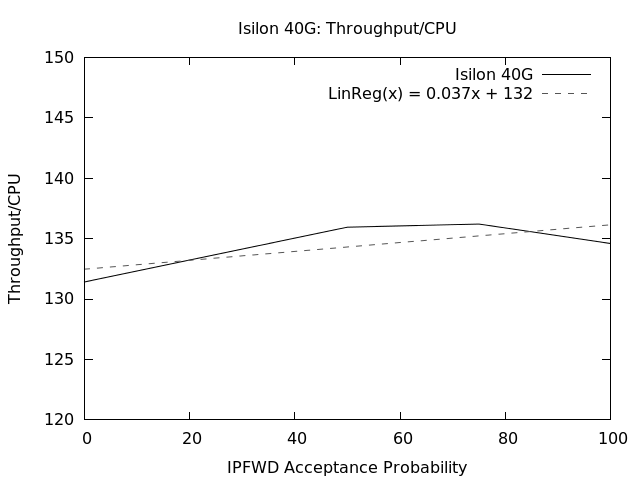
\includegraphics[width=0.45\textwidth]{toc_isilon40}
  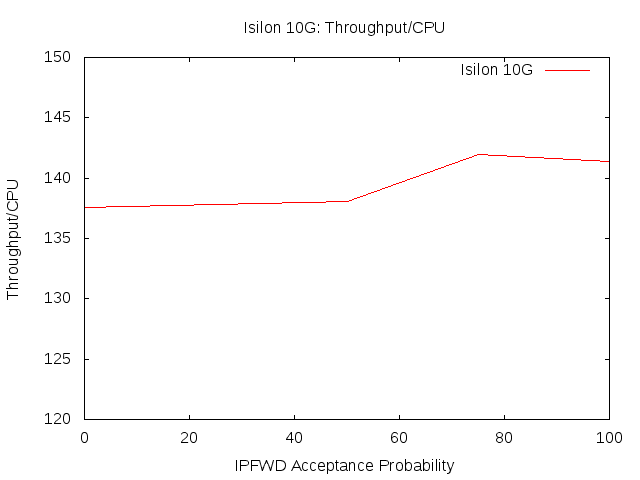
\includegraphics[width=0.45\textwidth]{toc_isilon10}
  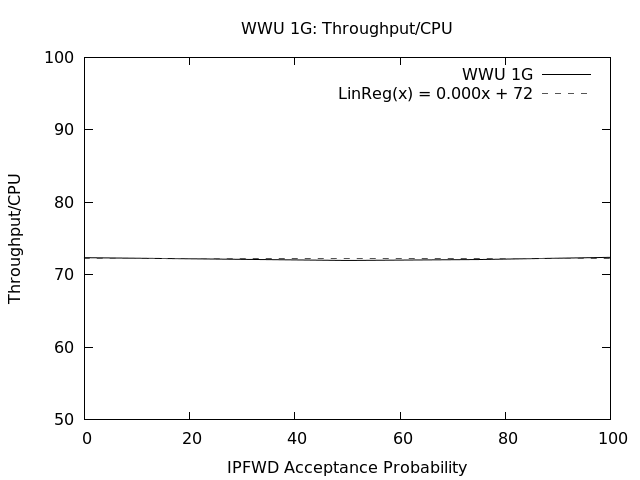
\includegraphics[width=0.45\textwidth]{toc_wwu1}
  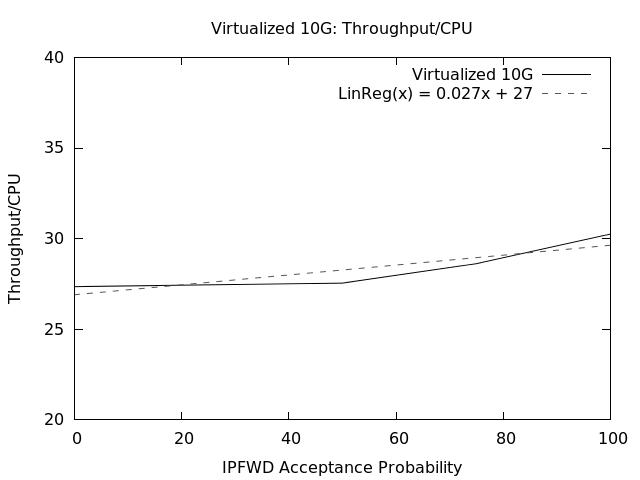
\includegraphics[width=0.45\textwidth]{toc_virtual10}
  \end{center}
  
  %  throughput & CPU
  \subsection{Throughput \& CPU}
  These graphs show the interaction between CPU utilization and network throughput for each system with respect to IPFWD's acceptance probability. The dashed lines are CPU utilization, solid is network throughput in Mb/second. Higher acceptance probability means a greater chance that a given packet is immediately accepted without further processing.
  
  \begin{center}
  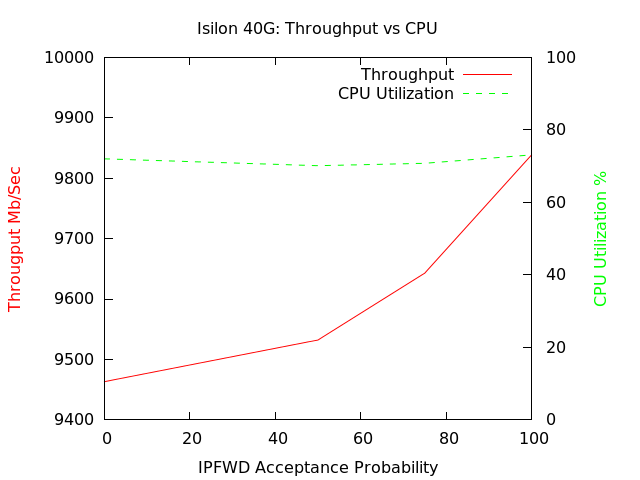
\includegraphics[width=0.45\textwidth]{isilon40_cpu}
  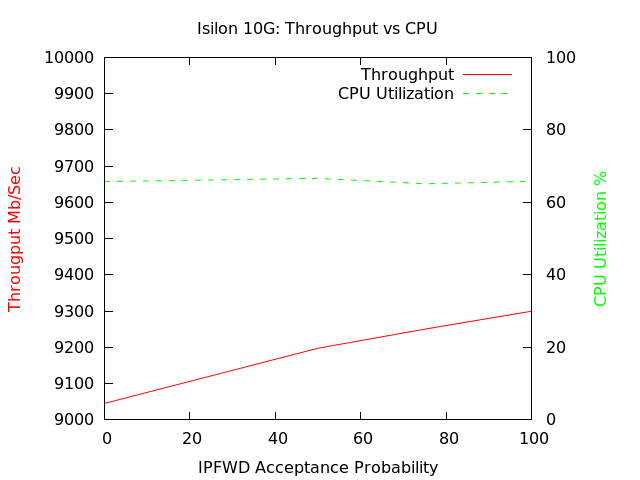
\includegraphics[width=0.45\textwidth]{isilon10_cpu}
  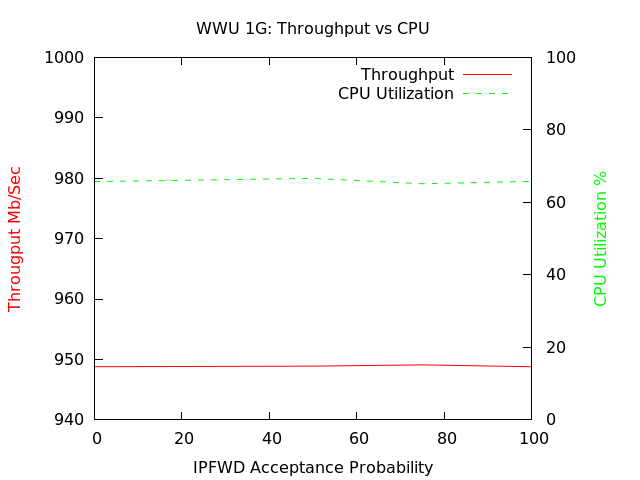
\includegraphics[width=0.45\textwidth]{wwu1_cpu}
  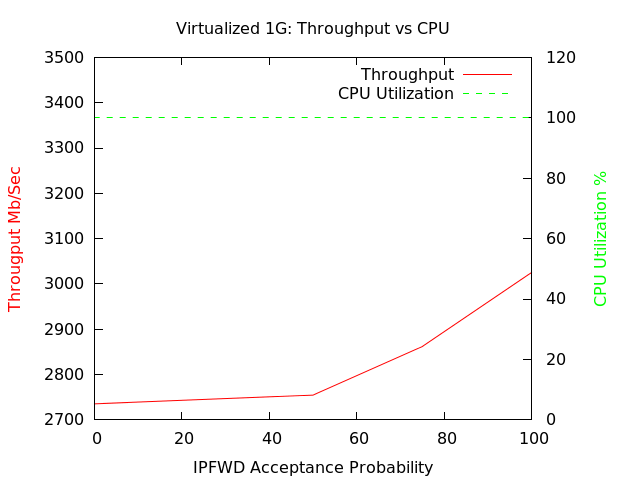
\includegraphics[width=0.45\textwidth]{virtual10_cpu}
  \end{center}

% Difference in results between CPU and throughput bound systems
  \subsection{Discussion} 

  All the systems tested can be broadly categorized into two groups: CPU bound
  and NIC throughput bound. We can see that IPFWD affects performance
  positively but differently for both types. 

  In CPU bound systems, IPFWD reduces the number of cycles it takes to process
  each packet, allowing more packets to be processed in the same time and
  increasing throughput. This is shown most clearly in the Virtualized system
  tests, which have the weakest CPU but 10Gb Ethernet NICs. Regardless of test
  type, the receiving system is always at 100\% CPU utilization. However, as
  the probability to accept increases in IPFWD the throughput also increases.
  This clearly shows that IPFWD decreases the CPU load required to process
  incoming traffic.

  In NIC throughput bound systems, reducing the number of CPU cycles to process
  packets will not increase throughput. However, IPFWD still reduces CPU load
  which allows more cycles to be dedicated to other system processes. This is
  more difficult to see in the test results, particularly since the CPU
  measurement tools are inherently imprecise and difficult to compare between
  systems.


\section{Related Work}
% Cisco and Juniper routers

Firewall decision trees? (Complete Redundancy Detection)

% Machine learning firewalls


\section{Future Work}
% Firewall rule reordering so we can "fail as early as possible"
Ideally, a whitelist firewall's rule set would be constructed so that the most
commonly applied matches are reached earlier rather than later. IPFWD
accomplishes this task by artificial early stopping. Firewall rule reordering
is a could be another solution to this problem. Given logs of common network
traffic for the system, statistical analysis could show which rules are matched
more often than others. With this information, the rule set could be reordered
so that the most commonly applied rules are earliest.


\section{Conclusion}
% What performance benefit do we get?

% What security cost is there?

% Why is this useful?

% Why is this important?


% if have a single appendix:
%\appendix[Proof of the Zonklar Equations]
% or
%\appendix  % for no appendix heading
% do not use \section anymore after \appendix, only \section*
% is possibly needed

% use appendices with more than one appendix
% then use \section to start each appendix
% you must declare a \section before using any
% \subsection or using \label (\appendices by itself
% starts a section numbered zero.)
%


\appendices
\section{Additional Figures}
Some text for the appendix.

% use section* for acknowledgement
\section*{Acknowledgment}


The authors would like to thank...


% Can use something like this to put references on a page
% by themselves when using endfloat and the captionsoff option.
\ifCLASSOPTIONcaptionsoff
  \newpage
\fi



% trigger a \newpage just before the given reference
% number - used to balance the columns on the last page
% adjust value as needed - may need to be readjusted if
% the document is modified later
%\IEEEtriggeratref{8}
% The "triggered" command can be changed if desired:
%\IEEEtriggercmd{\enlargethispage{-5in}}

% references section

% can use a bibliography generated by BibTeX as a .bbl file
% BibTeX documentation can be easily obtained at:
% http://www.ctan.org/tex-archive/biblio/bibtex/contrib/doc/
% The IEEEtran BibTeX style support page is at:
% http://www.michaelshell.org/tex/ieeetran/bibtex/
%\bibliographystyle{IEEEtran}
% argument is your BibTeX string definitions and bibliography database(s)
%\bibliography{IEEEabrv,../bib/paper}
%
% <OR> manually copy in the resultant .bbl file
% set second argument of \begin to the number of references
% (used to reserve space for the reference number labels box)
\begin{thebibliography}{1}

\bibitem{IEEEhowto:kopka}
H.~Kopka and P.~W. Daly, \emph{A Guide to \LaTeX}, 3rd~ed.\hskip 1em plus
  0.5em minus 0.4em\relax Harlow, England: Addison-Wesley, 1999.

% http://www.netperf.org/svn/netperf2/tags/netperf-2.7.0/doc/netperf.html#CPU-Utilization

\end{thebibliography}

% biography section
% 
% If you have an EPS/PDF photo (graphicx package needed) extra braces are
% needed around the contents of the optional argument to biography to prevent
% the LaTeX parser from getting confused when it sees the complicated
% \includegraphics command within an optional argument. (You could create
% your own custom macro containing the \includegraphics command to make things
% simpler here.)
%\begin{biography}[{\includegraphics[width=1in,height=1.25in,clip,keepaspectratio]{mshell}}]{Michael Shell}
% or if you just want to reserve a space for a photo:


% that's all folks
\end{document}


% NOTES
%==========================================================
% needed in second column of first page if using \IEEEpubid
%\IEEEpubidadjcol

% An example of a floating figure using the graphicx package.
% Note that \label must occur AFTER (or within) \caption.
% For figures, \caption should occur after the \includegraphics.
% Note that IEEEtran v1.7 and later has special internal code that
% is designed to preserve the operation of \label within \caption
% even when the captionsoff option is in effect. However, because
% of issues like this, it may be the safest practice to put all your
% \label just after \caption rather than within \caption{}.
%
% Reminder: the "draftcls" or "draftclsnofoot", not "draft", class
% option should be used if it is desired that the figures are to be
% displayed while in draft mode.
%
%\begin{figure}[!t]
%\centering
%\includegraphics[width=2.5in]{myfigure}
% where an .eps filename suffix will be assumed under latex, 
% and a .pdf suffix will be assumed for pdflatex; or what has been declared
% via \DeclareGraphicsExtensions.
%\caption{Simulation Results}
%\label{fig_sim}
%\end{figure}

% Note that IEEE typically puts floats only at the top, even when this
% results in a large percentage of a column being occupied by floats.


% An example of a double column floating figure using two subfigures.
% (The subfig.sty package must be loaded for this to work.)
% The subfigure \label commands are set within each subfloat command, the
% \label for the overall figure must come after \caption.
% \hfil must be used as a separator to get equal spacing.
% The subfigure.sty package works much the same way, except \subfigure is
% used instead of \subfloat.
%
%\begin{figure*}[!t]
%\centerline{\subfloat[Case I]\includegraphics[width=2.5in]{subfigcase1}%
%\label{fig_first_case}}
%\hfil
%\subfloat[Case II]{\includegraphics[width=2.5in]{subfigcase2}%
%\label{fig_second_case}}}
%\caption{Simulation results}
%\label{fig_sim}
%\end{figure*}
%
% Note that often IEEE papers with subfigures do not employ subfigure
% captions (using the optional argument to \subfloat), but instead will
% reference/describe all of them (a), (b), etc., within the main caption.


% An example of a floating table. Note that, for IEEE style tables, the 
% \caption command should come BEFORE the table. Table text will default to
% \footnotesize as IEEE normally uses this smaller font for tables.
% The \label must come after \caption as always.
%
%\begin{table}[!t]
%% increase table row spacing, adjust to taste
%\renewcommand{\arraystretch}{1.3}
% if using array.sty, it might be a good idea to tweak the value of
% \extrarowheight as needed to properly center the text within the cells
%\caption{An Example of a Table}
%\label{table_example}
%\centering
%% Some packages, such as MDW tools, offer better commands for making tables
%% than the plain LaTeX2e tabular which is used here.
%\begin{tabular}{|c||c|}
%\hline
%One & Two\\
%\hline
%Three & Four\\
%\hline
%\end{tabular}
%\end{table}


% Note that IEEE does not put floats in the very first column - or typically
% anywhere on the first page for that matter. Also, in-text middle ("here")
% positioning is not used. Most IEEE journals use top floats exclusively.
% Note that, LaTeX2e, unlike IEEE journals, places footnotes above bottom
% floats. This can be corrected via the \fnbelowfloat command of the
% stfloats package.

